\documentclass[../main.tex]{subfiles}

\begin{document}
    \begin{figure}[H]
        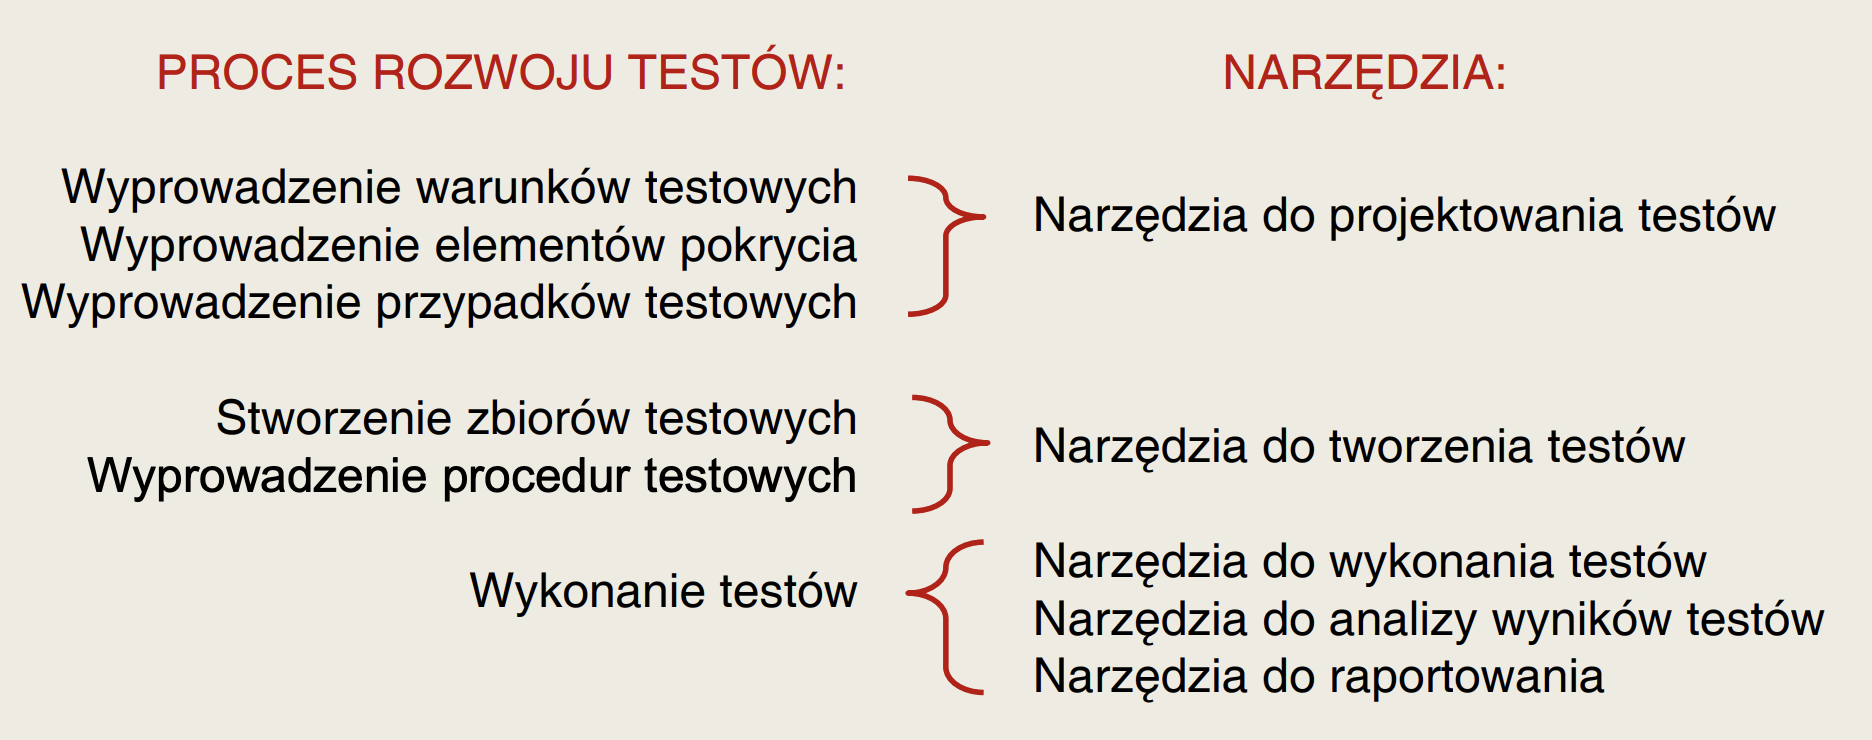
\includegraphics[width=\linewidth]{auttest.png}
    \end{figure}

    \textbf{Efekt próbnika (probe effect)} - niezamierzony wpływ na zachowanie systemu spowodowany pomiarami tego systemu.
    Narzędzie które wpływa na wynik testu nazywamy \textbf{inwazyjnym}.

    \subsection{ Generyczna architektura automatyzacji testów}
    \begin{figure}[H]
        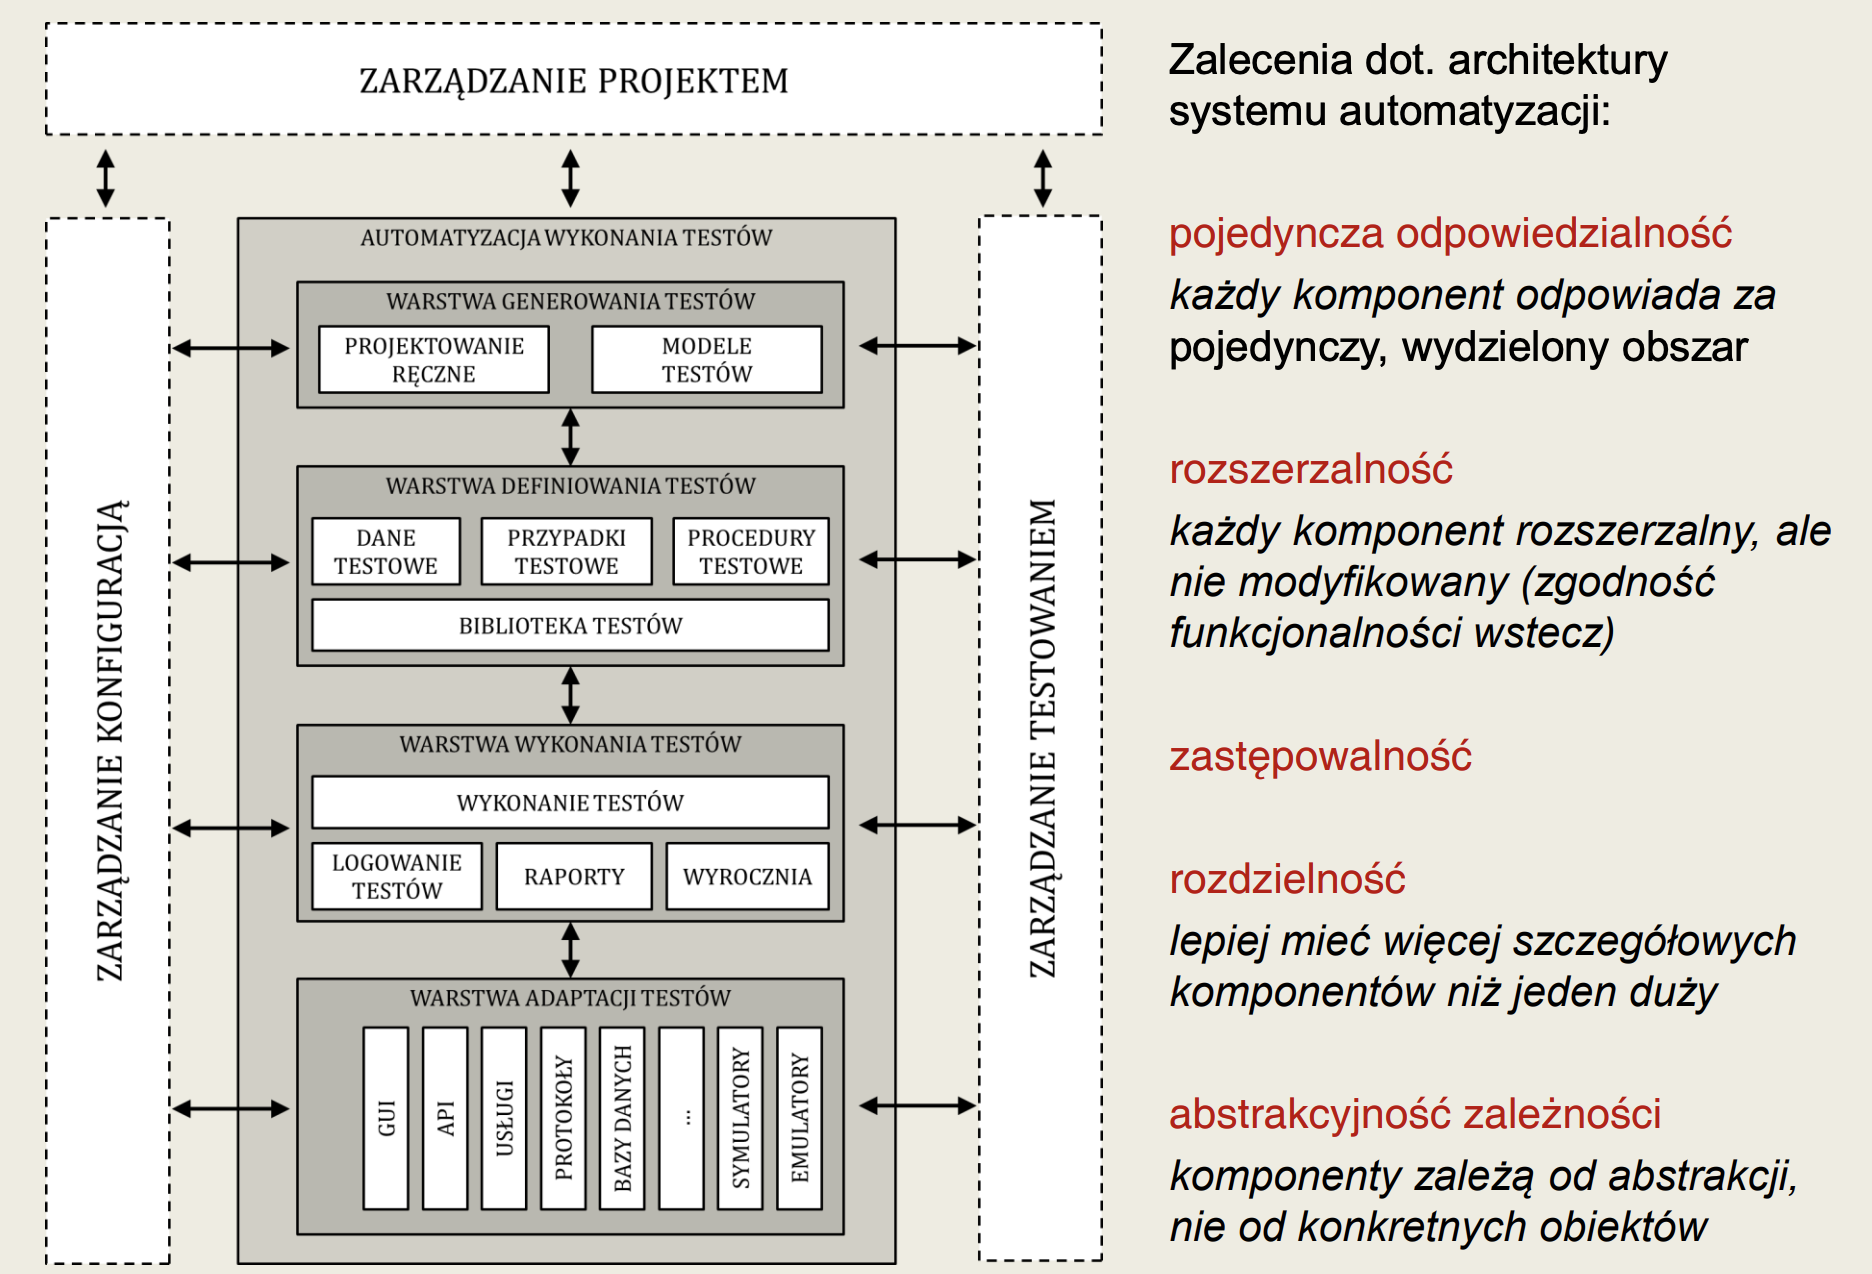
\includegraphics[width=\linewidth]{genaut.png}
    \end{figure}

    \subsection{Automatyczna generacja danych testowych}
    \begin{table}[H]
        \begin{center}
            \begin{tabular}{p{8cm} p{8cm}}
                \begin{itemize}
                    \item metoda losowa
                    \item generacja z rozkładu prawdopodobieństwa
                    \item generacja z modelu
                \end{itemize}
                &
                \begin{itemize}
                    \item generacja na podstawie symbolicznego wykonania kodu
                    \item generacja metodyczna (np. pair-wise)
                    \item generacja na podstawie danych zewnętrzych
                \end{itemize}
            \end{tabular}
        \end{center}
    \end{table}

    \subsection{Techniki automatyzacji testów}
    \begin{tabular}{| p{5cm} || p {5cm} | p{5cm} |}
        \hline
        \textbf{Technika} & \textbf{Zalety} & \textbf{Wady}\\
        \hline
        \hline
        \textbf{nagraj i odtwórz} &
        stosowalne na poziomie GUI lub API, łatwe do konfiguracji i użycia, nie
        wymaga znajomości języków
        &
        trudne w utrzymaniu, problemy gdy potrzeba czasu na odpowiedź systemu\\
        \hline
        \textbf{skrypty linearne} &
        brak żmudnych i kosztownych przygotowań, znajomość programowania niekonieczna gdy
        skrypt tworzony automatycznie
        &
        koszt automatyzacji liniowy ze względu na liczbę skryptów; trudne i kosztowne w utrzymaniu\\
        \hline
        \textbf{skrypty zorganizowane} &
        redukcja kosztów utrzymania, zmniejszenie kosztu automatyzacji nowych testów
        &
        zwiększone koszty początkowe tworzenia reużywalnych skryptów; wymaga umiejętności
        programowania\\
        \hline
        \textbf{data-driven testing} &
        niski koszt dodania testu; nie wymaga znajomości programowania; tanie w utrzymaniu
        &
        ograniczona możliwość przeprowadzania testów negatywnych\\
        \hline
        \textbf{keyword-driven testing} &
        tanie w utrzymaniu; swoboda w tworzeniu testów
        &
        kosztowna implementacja słów kluczowych; trudność w doborze właściwych słów\\
        \hline
    \end{tabular}

    \subsection{Testowanie oparte na modelu (MBT)}

    \begin{itemize}
        \item \textbf{Podstawowa idea: ulepszyć jakość i efektywność} projektu i implementacji testów przez:
        \begin{itemize}
            \item projekt wyczerpującego modelu MBT, zwykle z użyciem narzędzi,
            \item użycie modelu jako specyfikacji projektu testów, pozwalającego na automatyczną generację przypadków testowych z modelu
        \end{itemize}
        \item \textbf{Rodzaje modeli}: strukturalne, behawioralne, danych.
    \end{itemize}

    \begin{table}[H]
        \begin{center}
            \begin{tabular}{p{8cm} p{8cm}}
                \textbf{Efektywność} & \textbf{Wydajność}\\
                \begin{itemize}
                    \item modelowanie ułatwia \textbf{komunikację} z interesariuszami
                    \item \textbf{zrozumienie}
                    \item \textbf{łatwiejsze zaangażowanie} interesariuszy modelem
                    \item \textbf{łatwa identyfikacja „problematycznych” części systemu}
                    \item \textbf{wczesna generacja i analiza przypadków testowych} - możliwe przed stworzeniem systemu
                \end{itemize}
                &
                \begin{itemize}
                    \item \textbf{wczesne unikanie defektów} - weryfikacja wymagań
                    \item \textbf{możliwe reużycie} artefaktów MBT
                    \item \textbf{automatyzacja} - np. generacja testaliów
                    \item \textbf{adaptacja do zmian} - różne suity testów mogą być generowane z tego samego modelu
                    \item \textbf{redukcja kosztów przy zmianie wymagań} - MBT pomaga zredukować koszty utrzymania gdy
                    zmieniają się wymagania, bo model MBT dostarcza „single point of maintenance”
                \end{itemize}\\
            \end{tabular}
        \end{center}
    \end{table}


    \begin{table}[H]
        \begin{center}
            \begin{tabular}{| p{8cm} | p{8cm} |}
                \hline
                \multicolumn{2}{|c|}{\textbf{Kryteria wyboru testów}}\\
                \hline
                \textbf{Oparte na pokryciu} & \textbf{Inne}\\
                \hline
                \begin{itemize}
                    \item \textbf{Wymagania połączone z modelem} - elementy modelu są połączone z wybranymi
                    wymaganiami. Pełne pokrycie wymagań odpowiada zestawowi testów całkowicie pokrywających wybrany zbiór wymagań.

                    \item \textbf{Elementy modelu MBT} - bazuje na \textbf{wewnętrznej strukturze modelu}. Definiuje się elementy
                    pokrycia, a testy powinny je pokrywać.

                    \item \textbf{Oparte na danych} - związane są z takimi technikami projektowania testów jak:
                    \begin{itemize}
                        \item podział na \textbf{klasy równoważności}
                        \item analiza \textbf{wartości} brzegowych
                        \item testy kombinatoryczne (np. pair-wise)
                    \end{itemize}
                \end{itemize}
                &
                \begin{itemize}
                    \item \textbf{Losowe} - polega na \textbf{losowym przechodzeniu przez model}, wszystkie przejścia są równo
                    prawdopodobne. \textbf{W podejściu stochastycznym} wybór oparty o \textbf{rozkład prawdopodobieństwa}. Model reprezentuje profil
                    użycia (tzw. \textbf{profil operacyjny}).
                    \item \textbf{Oparte na scenariuszu/wzorcu} - scenariuszem może być use case lub
                    scenariusz użycia; wzorzec = częściowo zdefiniowany scenariusz, który można
                    zastosować do modelu MBT aby wyprowadzić jeden lub wiele testów.
                    \item \textbf{Sterowane projektem} - podejście oparte na dodatkowej informacji projektowej, która została
                    dodana do modelu aby wspierać zarządzanie testami i/lub aby osiągnąć specificzne cele testowe w projekcie.
                \end{itemize}\\
                \hline
            \end{tabular}
        \end{center}
    \end{table}
\end{document}